\chapter{User Documentation} % User guide
\label{ch:user}

\section{Overview}

A user upon opening the application gets the details of the status of the application..
If the user wants to upload new data it can navigate to the upload tab respectively. Otherwise the user 
can choose the see the visualizations of the system based on existing data.

\begin{table}[H]
	\centering
	\begin{tabular}{ | m{0.25\textwidth} | m{0.65\textwidth} | }
		\hline
		\textbf{Component} & \textbf{Description} \\
		\hline \hline
		\emph{Dashboard} & Summarized information and status. \\
		\hline
		\emph{Upload} & Data uploading functionality sorted by type of data. \\
		\hline
		\emph{Analysis} & Visualizations of different data models implemented in the system \\
		\hline
	\end{tabular}
	\caption{Visual Composition of the Application}
	\label{tab:overall}
\end{table}


\begin{figure}[H]
	\centering
	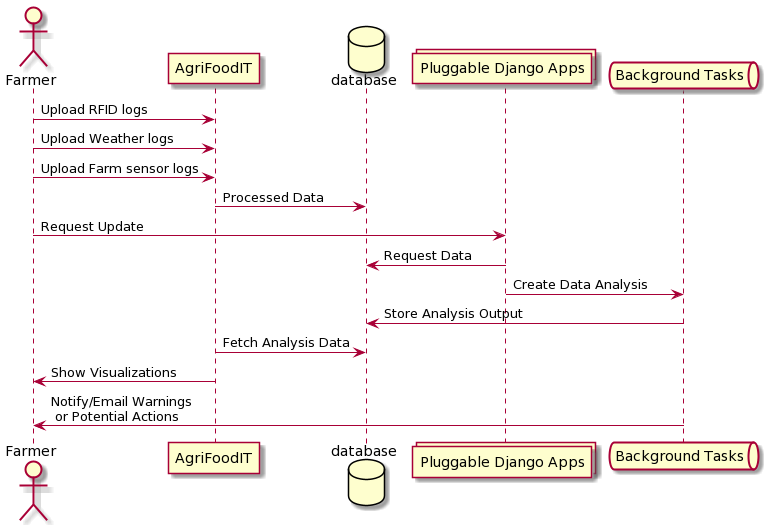
\includegraphics[width=1.0\textwidth]{workflow}
	\caption{Request/Response cycle overview and the communication between components}
	\label{fig:overview_uml}
\end{figure}

\section{Dashboard}

A user upon opening the application gets the details of the status of the application.
Currently the user is told about the last upload of data. If the user wishes to upload new
data they can press on the blue card and the application will redirect to the respective upload
webpage.

\begin{figure}[H]
	\centering
	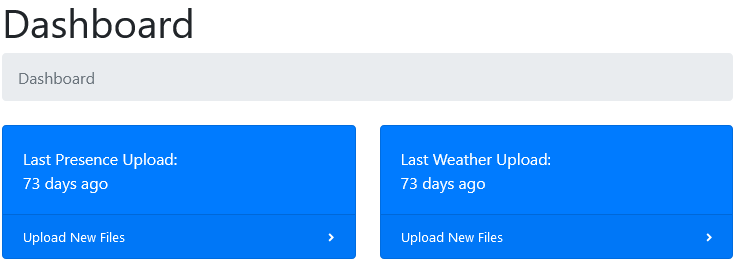
\includegraphics[width=1.0\textwidth]{main_dashboard}
	\caption{Landing page of the application}
	\label{fig:landing-page}
\end{figure}

\begin{figure}[H]
	\centering
	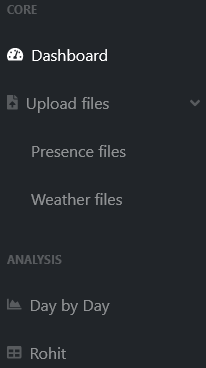
\includegraphics[height=200px]{navigation_bar}
	\caption{Navigation bar on the left of the application}
	\label{fig:navigation}
\end{figure}

\section{Upload}

Each type of data is uploaded on it's each separate page. Each page implements
the same features for file handling and processing. Files can be dragged and dropped on
to the upload area. Otherwise the user can press on the area to have a file selector dialog pop up
to select files from the filesystem. Data files of other types
are rejected with a cross and accepted files show a tick after successfully uploading.
On hovering above the rejected file one can see a error message describing why the file
was rejected by the application.

\begin{figure}[H]
	\centering
	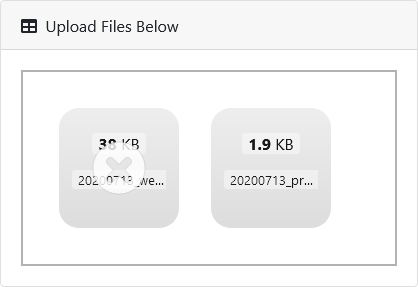
\includegraphics[width=0.9\linewidth]{upload_area}
	\caption{Upload Area with rejected and accepted file}
	\label{fig:upload-area}
\end{figure}

The files are put into a background processing queue which processed each line in the uploaded
files. As the files get processed their status is updated. The background
process manager Celery shows the logs as it receives each file for processing.
\begin{figure}[H]
	\centering
	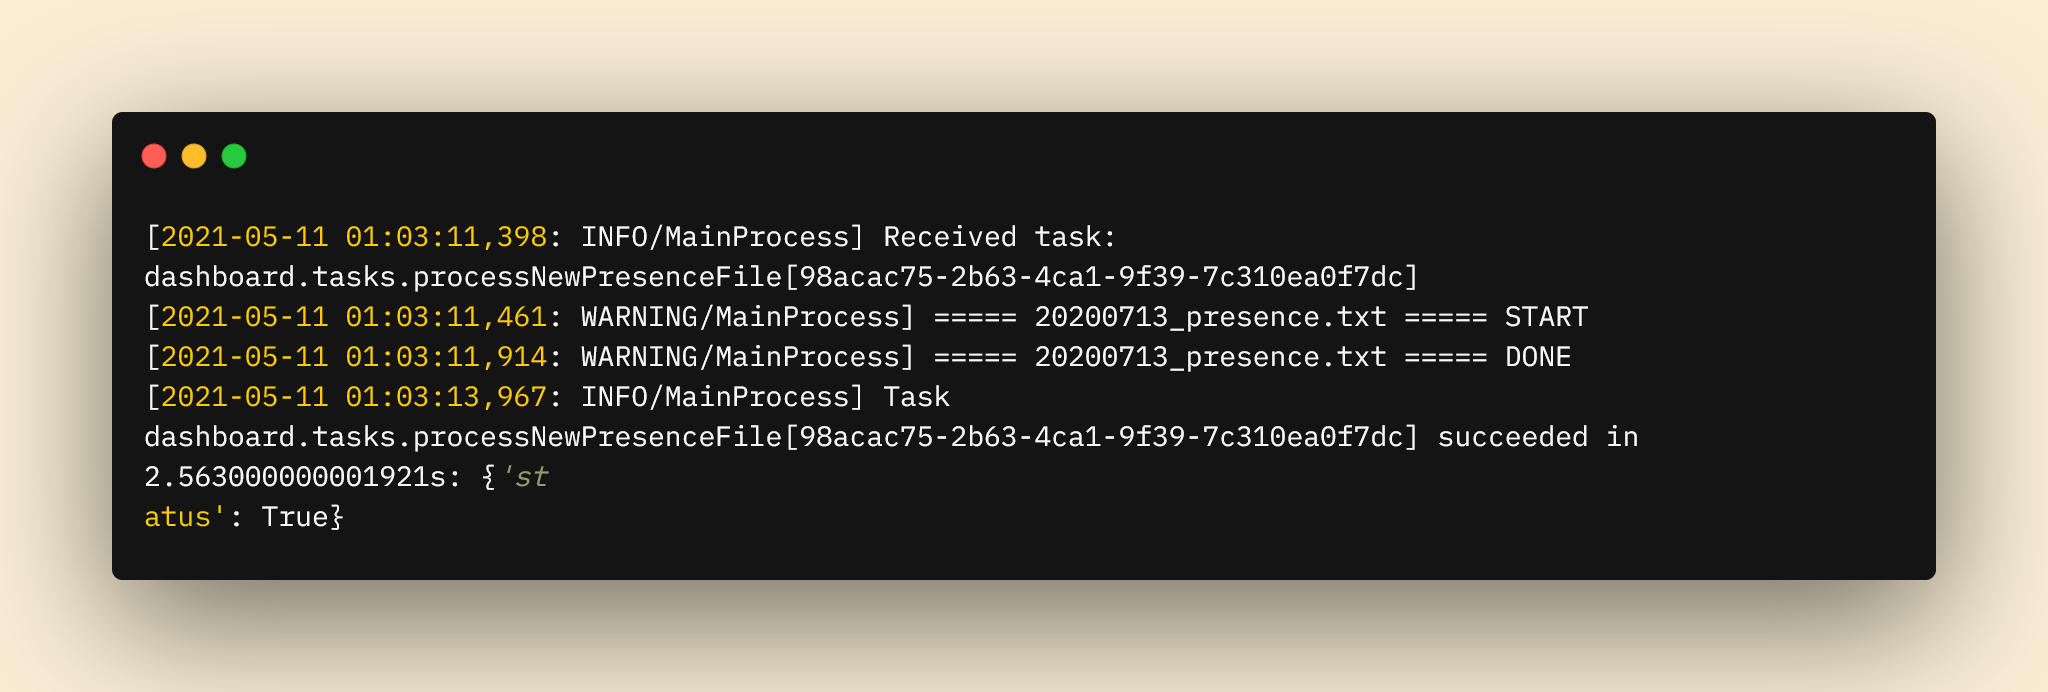
\includegraphics[width=1.0\linewidth]{celery_task_log}
	\caption{Process a single presence.txt file}
	\label{fig:celery-task-log}
\end{figure}

The files table shows all the uploaded files and it has
the following features:
\begin{enumerate}
	\item Search across all 4 columns.
	\item Sort ascending/descending by any single column.
	\item Change the amount of rows between 10, 25, 50, 100.
\end{enumerate}

\begin{figure}[H]
	\centering
	\subfigure[Files in Queue]{
		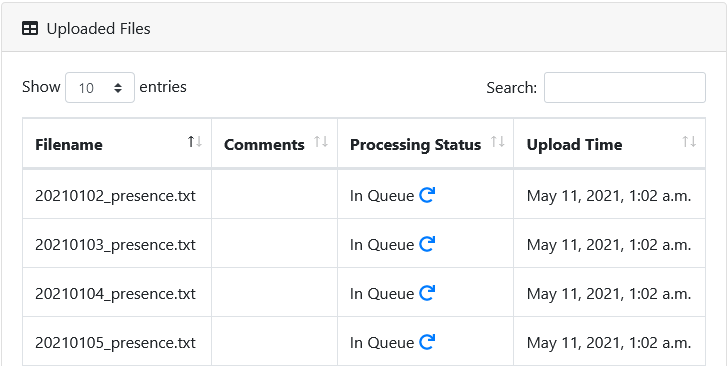
\includegraphics[width=1.0\linewidth]{upload_table_unprocessed}
		}

	\subfigure[Files completely processed]{
		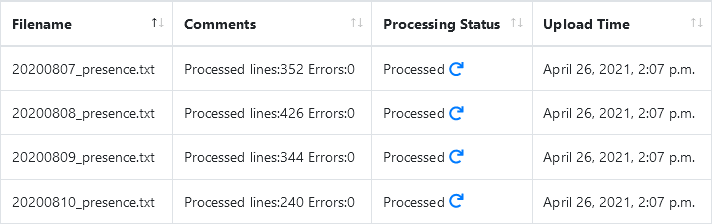
\includegraphics[width=1.0\linewidth]{upload_table_processed}
		}
	\caption{Files table with unprocessed and processed files}
	\label{fig:upload-table}
\end{figure}

\section{Analysis}

The analysis run automatically after uploading of new data. They can also
run at a pre-defined interval. For proof of concept 2 different visualizations
are implemented. A simple Temperature/Humidity graph and a complex analysis model.
Every graph implements the following functionality:
\begin{enumerate}
	\item Move around the graph interactively (Zoom/Pan).
	\item Take screenshot of the graph.
	\item Box selection and lasso selection.
\end{enumerate}

\begin{figure}[H]
	\centering
	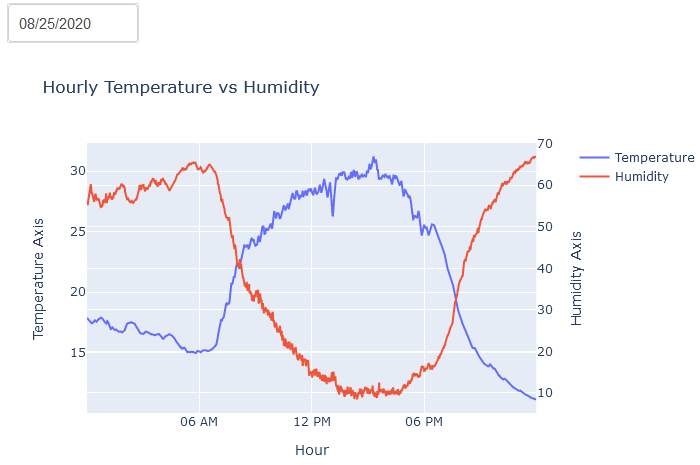
\includegraphics[width=1.0\linewidth]{simple_analysis}
	\caption{Plotly Temperature vs Humidity graph}
	\label{fig:simple-analysis}
\end{figure}

\begin{figure}[H]
	\centering
	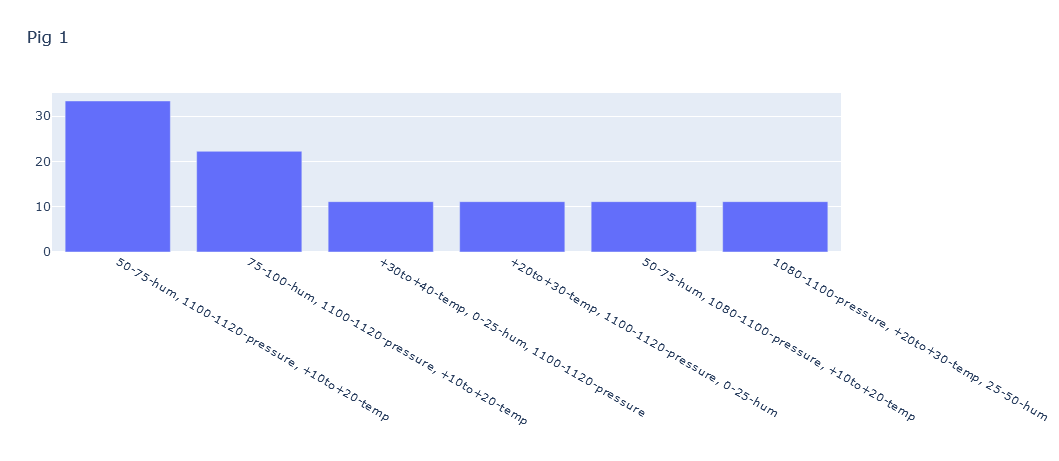
\includegraphics[width=1.0\linewidth]{rohit_analysis}
	\caption{Advanced analysis visualization after background processing}
	\label{fig:rohit-analysis}
\end{figure}